\documentclass[11pt]{article}

%%%%%%%%%%%%%%Include Packages%%%%%%%%%%%%%%%%%%%%%%%%%%
\usepackage{xcolor}
\usepackage{mathtools}
\usepackage[a4paper, total={6in, 8in}, margin=1.25in]{geometry}
\usepackage{amsmath}
\usepackage{amssymb}
\usepackage{paralist}
\usepackage{rsfso}
\usepackage{amsthm}
\usepackage{wasysym}
\usepackage[inline]{enumitem}   
\usepackage{hyperref}
\usepackage{tocloft}
\usepackage{titlesec}
\usepackage{colortbl}
\usepackage{wrapfig}
\usepackage{pdfpages}
%%%%%%%%%%%%%%%%%%%%%%%%%%%%%%%%%%%%%%%%%%%%%%%%%%%%%%%%



\begin{document}

\begin{wrapfigure}[10]{r}{0.42\textwidth}
  \begin{center}
  \vspace{-15pt}
    \includegraphics[scale=0.38]{swingccw}
  \end{center}
\end{wrapfigure}
\Large \noindent \textbf{Physics 5A Discussion (Week 8)}\\
\normalsize
Department of Physics and Astronomy, UCLA\\
\noindent\rule{8cm}{0.4pt}\\
%\begin{center}
%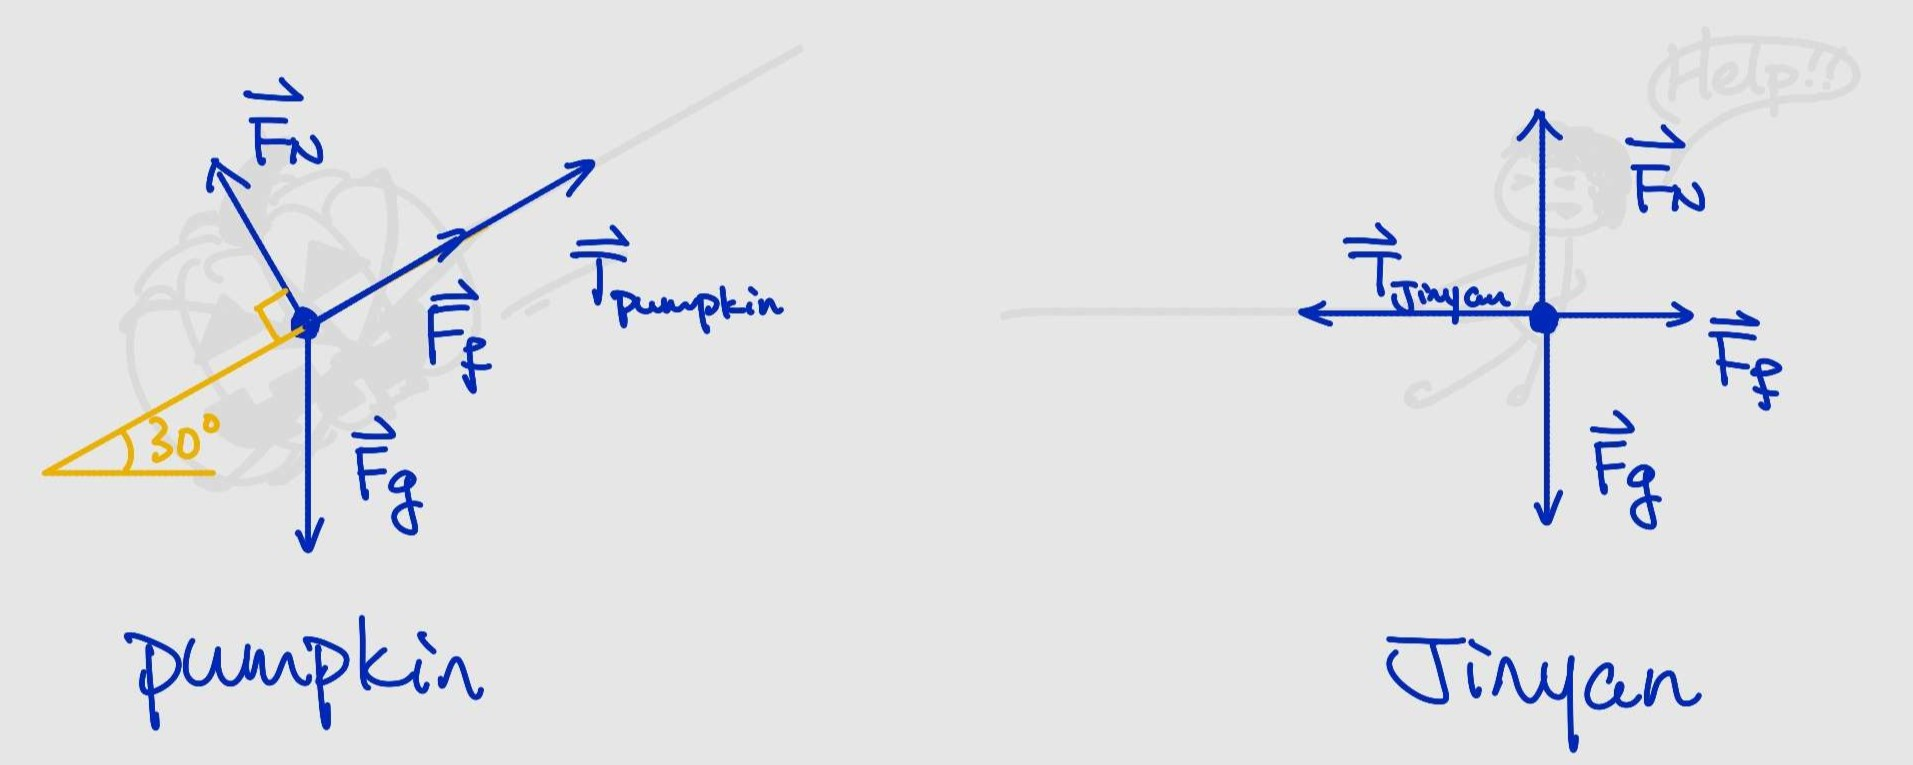
\includegraphics[scale=0.55]{pull}
%\end{center}
Jinyan is swinging a $2\, \text{kg}$ pumpkin in a huge circular path by using a rope attached to the pumpkin. The radius of the circular path is $R =1\,$m. He is trying to stop the pumpkin so he is making it spin slower. At time $t=0$ seconds, the pumpkin is spinning with an angular velocity $\omega = 5$ rad/s counterclockwise. He is able to maintain a tangential acceleration $a_t = -1$ m/s$^2$. \\
\hfill\break

\noindent\textbf{Part (a)} Find the centripetal acceleration and centripetal force that the pumpkin experiences at time $t = 0$ seconds. (\textit{Hint: First find the tangential speed at time $t = 0$.})

\hfill\break\hfill\break
\hfill\break\hfill\break
\hfill\break\hfill\break

\noindent\textbf{Part (b)} Find the angular acceleration of the pumpkin.

\hfill\break\hfill\break
\hfill\break\hfill\break
\hfill\break\hfill\break

\noindent\textbf{Part (c)} Find the tangential speed and angular speed of the pumpkin as a function of time (that is, leaving $t$ as a variable in your final expression). 

\hfill\break\hfill\break
\hfill\break\hfill\break
\hfill\break\hfill\break

\noindent\textbf{Part (d)} Find the centripetal acceleration of the pumpkin as a function of time. 
\hfill\break\hfill\break
\hfill\break\hfill\break
\hfill\break\hfill\break

\newpage
\noindent\textbf{Part (e)} Last week, we found that the pumpkin has to go faster than $v_t = 3.13$ m/s. Find the time that the pumpkin will reach $v_t = 3.13$ m/s. 
\hfill\break\hfill\break
\hfill\break\hfill\break
\hfill\break\hfill\break

\noindent\textbf{Part (f)} Find the frequency and period of the circular motion at time $t = 0$ seconds. 
\hfill\break\hfill\break
\hfill\break\hfill\break
\hfill\break\hfill\break


At time $t = 0$ seconds, the center of mass of the pumpkin is located at $\vec{r}_p = (1,2)$ in meters, and the center of mass of Jinyan is located at $\vec{r}_m = (0,5)$ in meters. The pumpkin is $m_p=2$\,kg and Jinyan is $m_j=60$\,kg. Find the center of mass of the Jinyan-holding-the-pumpkin system, ignore the mass of the rope. 

\vfill
\begin{align*}
\mathbb{GOOD\ LUCK\ ON\ THE\ EXAM}.
\end{align*}

\newpage
Solutions:\\

\textbf{Part (a)}: The tangential speed at time $t= 0$ is $v_{t,0} = \omega R = 5$\,m/s. Then we can find the centripetal acceleration at time $t = 0$ seconds,
\begin{align*}
a_c = \frac{v_t^2}{R} = 25\,\text{m/s}^2\,.
\end{align*}
Centripetal force at time $t = 0$ is obtained from Newton's second law, 
\begin{align*}
F_c = ma_c = (2\,\text{kg}) \cdot (25\,\text{m/s}^2) = 50\,\text{N}\,.
\end{align*}

\textbf{Part (b)}: The angular acceleration of the pumpkin is a constant,
\begin{align*}
\alpha = \frac{a_t}{R} = -1 \,\text{rad/s}^2\,.
\end{align*}

\textbf{Part (c)}: The tangential speed as a function of time is 
\begin{align*}
v_t = v_{t,0} + a_t t = 5 -t\,,
\end{align*}
and the unit is meter per second. The angular speed of the pumpkin as a function of time is 
\begin{align*}
\omega = \omega_0 + \alpha t = 5 -t\,,
\end{align*}
and the unit is rad per second. It is a coincidence here $v_t = \omega$ numerically (because radius is $1$ meter), generally they have different numerical values. \\

\textbf{Part (d)}: The centripetal acceleration of the pumpkin is not a constant, because its tangential speed is changing, 
\begin{align*}
a_{c} = \frac{v_t^2}{R} = \frac{(5-t)^2}{1} = (5-t)^2\,,
\end{align*}  
with unit being m/s$^2$. \\

\textbf{Part (e)} We have found the tangential speed $v_t$ as a function of time, so we set $v_t = 3.13$\,m/s and find the time $t$, 
\begin{align*}
v_t = 5-t = 3.13\,,
\end{align*}
so we get $t = 1.87$ seconds. \\

\textbf{Part (f)} This is the same problem that we did last week. The period is defined by the time it takes to go one full circle, which corresponds to the angle $\theta = 2\pi$, or the distance traveled $d = 2\pi R$ being the circumference of the circle. We can find the period $T$ using either way, starting with the easy one, time is distance over velocity,
\begin{align*}
T = \frac{2\pi R}{v_t} = \frac{2\pi}{5} \,\text{s}= 1.26\,\text{s}\,.
\end{align*}
Or using the angle, again, time is angle over angular velocity, 
\begin{align*}
T = \frac{2\pi}{\omega} = \frac{2\pi}{5}\,\text{s} = 1.26\,\text{s}\,.
\end{align*}
Frequency is computed by taking the inverse of period, 
\begin{align*}
f = \frac{1}{T} = 0.793 \,\text{rev/s}
\end{align*}

\newpage
Center of mass is calculated using the following formula
\begin{align*}
\vec{r}_{\text{COM}} = \frac{\sum_i m_i \vec{r}_i}{\sum_i m_i}= \frac{m_p \vec{r}_p + m_j \vec{r}_j}{m_p + m_j} \,.
\end{align*}
This involves adding vectors, so we need to break it down to components. 
\begin{align*}
\vec{r}_{\text{COM}} &= \left(
\frac{(2\,\text{kg})\cdot (1\,\text{m})+(60\,\text{kg})\cdot (0\,\text{m}) }{(2\,\text{kg})+(60\,\text{kg})}\,,\ 
\frac{(2\,\text{kg})\cdot (2\,\text{m})+(60\,\text{kg})\cdot (5\,\text{m}) }{(2\,\text{kg})+(60\,\text{kg})} 
\right)= \left(\frac{1}{31}\,\text{m}\,, \ \frac{152}{31}\,\text{m}\right)\,.
\end{align*}


\end{document}


